\documentclass[a4paper, 12pt]{article}
\usepackage[top=1.8cm, bottom=1.8cm, left=1.5cm, right=1.5cm]{geometry}
\usepackage[utf8]{inputenc}
\usepackage{amsmath}
\usepackage{graphicx}
\usepackage{float}
\usepackage{pgfplots}
\pgfplotsset{compat=1.18}

\begin{document}
	\begin{center}
		Universidade Federal do Rio Grande do Norte
		
		Departamento de Engenharia da Computação e Automação  
		
		DCA3703 - Programação Paralela  
		
		\textbf{Tarefa 12: Avaliação da Escalabilidade}  
		
		\textbf{Aluno:} Daniel Bruno Trindade da Silva  
	\end{center}  
	
	\section{Introdução}  
	\hspace{.62cm}Este relatório tem como objetivo apresentar o conhecimento adquirido durante a realização da Tarefa 12 da disciplina de \textbf{Computação Paralela}. A atividade consistiu em avaliar a escalabilidade do programa desenvolvido na tarefa 11 (Simulador de velocidade de um fluido utilizando a equação de Navier-Stokes) utilizando o super computador NPAD da Universidade Federal do Rio Grande do Norte.  
	
	\section{Enunciado}    
	\hspace{.62cm} Avalie a escalabilidade do seu código de Navier-Strokes utilizando algum nó de computação do NPAD. Procure identificar gargalos de escalabilidade e reporte o seu progresso em versões sucessivas da evolução do código otimizado. Comente sobre a escalabilidade, a escalabilidade fraca e a escalabilidade fortes das versões.  
	
	\section{Desenvolvimento}
	\hspace{.62cm}Na Tarefa 11, desenvolvemos duas versões de um programa para simular a velocidade de um fluido: uma versão sequencial (serial) e outra paralelizada com OpenMP. Para a análise de escalabilidade, utilizamos a versão paralela. Foram realizados dois testes de escalabilidade:
	
	\begin{itemize}
		\item \textbf{Escalabilidade Forte} - Nesse teste, fixamos o tamanho do problema e aumentamos os recursos computacionais utilizados. Neste caso, foi feito um aumento gradual do número de \textit{threads} na execução. O código foi executado utilizando 1, 2, 4, 8, 16 e 32 \textit{threads}. A partir do tempo despendido em cada uma das execuções, podemos verificar como ficou a eficiência do programa.
		
		\item \textbf{Escalabilidade Fraca} - Para avaliarmos esse item, fixamos o poder computacional na utilização de 8 \textit{threads} e começamos a aumentar o tamanho da matriz tridimensional utilizada no problema. O código inicia com uma matriz 20x20x20 e, gradualmente, dobramos uma das dimensões: 20x20x40, 20x20x80, até 20x20x320. Com o tempo despendido em cada uma das execuções, podemos identificar se há um crescimento linear ou não, o que indicará se há uma boa escalabilidade fraca.
	\end{itemize}
	
	 Dessa forma, é possível avaliar o comportamento do programa em termos de escalabilidade forte, identificando possíveis gargalos e analisando o ganho de desempenho à medida que mais threads são utilizadas.
	 
	 \section{Resultados}
	 \subsection{Escalabilidade Forte}
	 \begin{table}[H]
	 	\centering
	 	\begin{tabular}{|c|c|c|c|c|c|c|}
	 		\hline
	 		\textbf{Threads} & 1 & 2 & 4 & 8 & 16 & 32 \\ \hline
	 		\textbf{Tempo (s)} & 1,365252 & 0,820158 & 0,532595 & 0,401583 & 0,356672 & 0,401173 \\ \hline
	 	\end{tabular}
	 	\caption{Resultados do teste de Escalabilidade Forte}
	 \end{table}
	 
	 \begin{figure}[H]
	 	\centering
	 	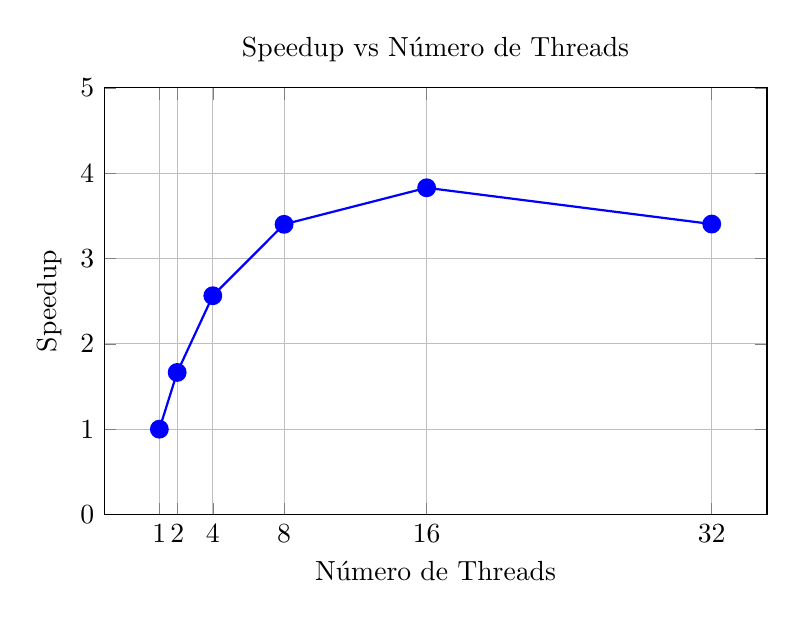
\begin{tikzpicture}
	 		\begin{axis}[
	 			title={Speedup vs Número de Threads},
	 			xlabel={Número de Threads},
	 			ylabel={Speedup},
	 			xtick={1,2,4,8,16,32},
	 			ymin=0, ymax=5,
	 			ytick={0,1,2,3,4,5},
	 			grid=both,
	 			width=10cm,
	 			height=7cm,
	 			mark size=3pt
	 			]
	 			\addplot[
	 			color=blue,
	 			mark=*,
	 			thick
	 			] coordinates {
	 				(1,1.000)
	 				(2,1.665)
	 				(4,2.564)
	 				(8,3.401)
	 				(16,3.829)
	 				(32,3.404)
	 			};
	 		\end{axis}
	 	\end{tikzpicture}
	 	\caption{Gráfico de Speedup conforme o número de threads.}
	 \end{figure}
	 
	 \subsection{Escalabilidade Fraca}
	 
	 \begin{table}[H]
	 	\centering
	 	\begin{tabular}{|c|c|c|c|c|c|c|}
	 		\hline
	 		\textbf{Dimensões da Matriz} & \textbf{20x20x20} & \textbf{20x20x40} & \textbf{20x20x80} & \textbf{20x20x160} & \textbf{20x20x320} \\
	 		\hline
	 		Tempo (s) & 0,401583 s & 0,726705 s & 1,375313 s & 2,675813 s & 5,387217 s \\
	 		\hline
	 	\end{tabular}
	 	\caption{Resultados do teste de escalabilidade fraca variando a dimensão da matriz.}
	 	\label{tab:esc_fraca}
	 \end{table}
	 
	 \begin{figure}[H]
	 	\centering
	 	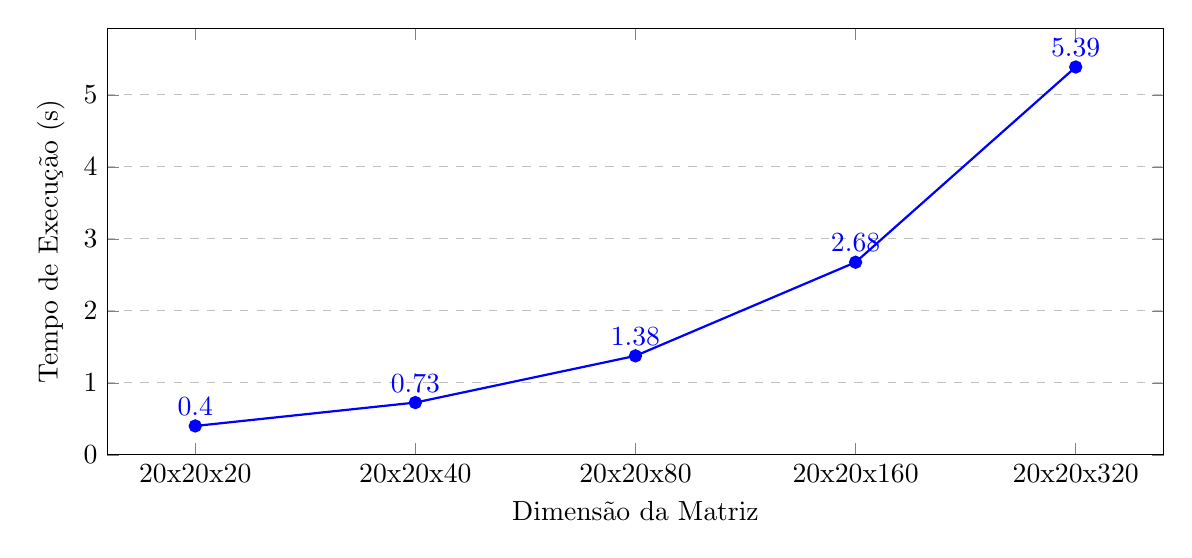
\begin{tikzpicture}
	 		\begin{axis}[
	 			width=15cm,
	 			height=7cm,
	 			xlabel={Dimensão da Matriz},
	 			ylabel={Tempo de Execução (s)},
	 			symbolic x coords={20x20x20, 20x20x40, 20x20x80, 20x20x160, 20x20x320},
	 			xtick=data,
	 			ymajorgrids=true,
	 			grid style=dashed,
	 			nodes near coords,
	 			nodes near coords align={vertical},
	 			ymin=0
	 			]
	 			\addplot[
	 			color=blue,
	 			mark=*,
	 			thick
	 			]
	 			coordinates {
	 				(20x20x20,0.401583)
	 				(20x20x40,0.726705)
	 				(20x20x80,1.375313)
	 				(20x20x160,2.675813)
	 				(20x20x320,5.387217)
	 			};
	 		\end{axis}
	 	\end{tikzpicture}
	 	\caption{Gráfico de escalabilidade fraca: tempo de execução conforme o aumento da dimensão da matriz.}
	 	\label{fig:esc_fraca}
	 \end{figure}
	 
	 
	 
	 

\end{document}
